% Self-Attention Mechanism Diagram
% Generated with TikZ

\documentclass[tikz,border=8pt]{standalone}
\usepackage{tikz}
\usetikzlibrary{calc,positioning,fit,backgrounds}
\usepackage{amsmath}

\begin{document}
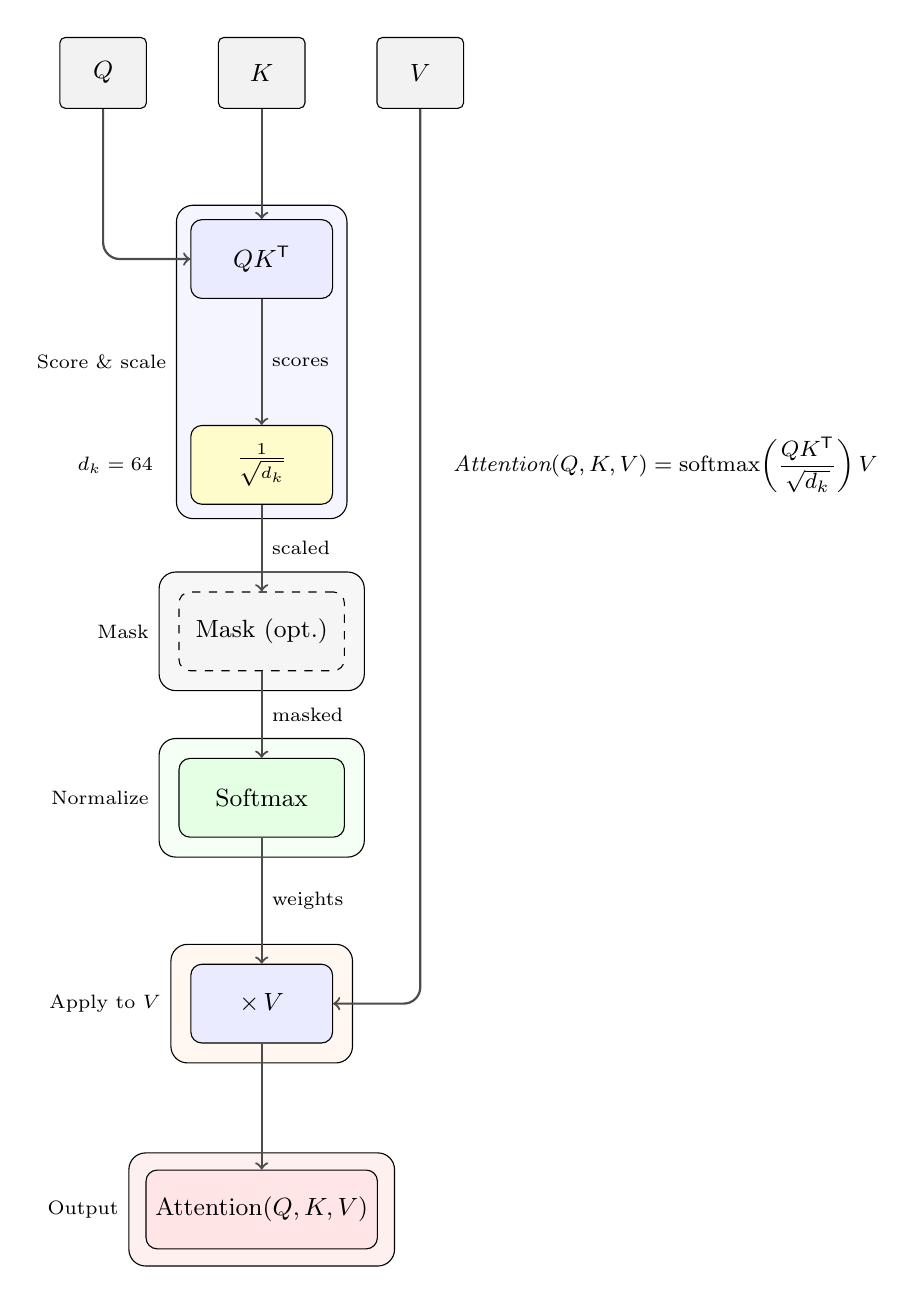
\begin{tikzpicture}[
        node distance=1.4cm,
        font=\small,
        input/.style={draw, rounded corners=2pt, minimum width=1.1cm, minimum height=0.9cm, fill=gray!10},
        op/.style={draw, rounded corners=4pt, minimum width=1.8cm, minimum height=1cm, fill=blue!8},
        mask/.style={draw, dashed, rounded corners=4pt, minimum width=2.1cm, minimum height=1cm, fill=gray!8},
        soft/.style={draw, rounded corners=4pt, minimum width=2.1cm, minimum height=1cm, fill=green!10},
        output/.style={draw, rounded corners=4pt, minimum width=2.1cm, minimum height=1cm, fill=red!10},
        arrow/.style={->, thick, draw=black!70},
        brace/.style={decorate, decoration={brace, amplitude=5pt}},
        dot/.style={circle, inner sep=2pt, fill=black!60, draw=none}
    ]

    % Inputs (horizontal row)
    \matrix[column sep=0.9cm] (inputs) {
        \node[input] (Q) {$Q$}; &
        \node[input] (K) {$K$}; &
        \node[input] (V) {$V$};   \\
    };

    % Score path
    \node[op, below=1.4cm of K] (mult) {$QK^{\mathsf T}$};
    \node[op, below=1.6cm of mult, fill=yellow!20] (scale) {$\frac{1}{\sqrt{d_k}}$};
    \node[mask, below=1.1cm of scale] (mask) {Mask (opt.)};
    \node[soft, below=1.1cm of mask] (softmax) {Softmax};

    % Value path
    \node[op, below=1.6cm of softmax] (weightv) {$\times\,V$};
    \node[output, below=1.6cm of weightv] (out) {$\text{Attention}(Q,K,V)$};

    % Lines
    \draw[arrow,rounded corners=6pt] (Q.south) |- (mult.west);
    \draw[arrow] (K.south) -- (mult.north);
    \draw[arrow] (mult) -- node[right, font=\scriptsize] {scores} (scale);
    \draw[arrow] (scale) -- node[right, font=\scriptsize] {scaled} (mask);
    \draw[arrow] (mask) -- node[right, font=\scriptsize] {masked} (softmax);
    \draw[arrow] (softmax) -- node[right, font=\scriptsize] {weights} (weightv);
    \draw[arrow,rounded corners=6pt] (V.south) |- (weightv.east);
    \draw[arrow] (weightv) -- (out);

    % Formula annotation
    \node[right=1.4cm of scale, align=center, font=\footnotesize\itshape] {
        $\text{Attention}(Q,K,V) = \operatorname{softmax}\!\left(\dfrac{QK^{\mathsf T}}{\sqrt{d_k}}\right)V$
    };

    % dk note
    \node[left=0.35cm of scale, font=\scriptsize, fill=white] {$d_k = 64$};

    % Grouping boxes (visual scaffolding)
    \begin{pgfonlayer}{background}
        \node[draw, rounded corners=6pt, fill=blue!4, fit=(mult) (scale), inner sep=5pt, label={[font=\scriptsize]left:Score \& scale}] {};
        \node[draw, rounded corners=6pt, fill=gray!6, fit=(mask), inner sep=7pt, label={[font=\scriptsize]left:Mask}] {};
        \node[draw, rounded corners=6pt, fill=green!4, fit=(softmax), inner sep=7pt, label={[font=\scriptsize]left:Normalize}] {};
        \node[draw, rounded corners=6pt, fill=orange!6, fit=(weightv), inner sep=7pt, label={[font=\scriptsize]left:Apply to $V$}] {};
        \node[draw, rounded corners=6pt, fill=red!6, fit=(out), inner sep=6pt, label={[font=\scriptsize]left:Output}] {};
    \end{pgfonlayer}

\end{tikzpicture}
\end{document}
